\subsection{Transformadores trifásicos}
La transformación de tensiones y corrientes en los sistemas trifásicos, según lo visto en la materia \materia, consiste en emplear un núcleo magnético en el que se incluyen los devanados necesarios. El núcleo de hierro visto en la figura \ref{fig:trafo-trifasico} está formado por tres columnas iguales sobre las que se arrollan las espiras del \textbf{devanado primario y secundario de cada fase por cada columna}.

\begin{figure}[H]
	\centering
	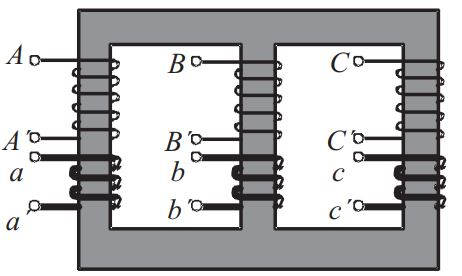
\includegraphics[width = .4\linewidth]{trafo-trifasico}
	\caption{Circuito magnético de un transformador trifásico.}
	\label{fig:trafo-trifasico}
\end{figure}

\subsubsection{Construcción a partir de tres trafos monofásicos}

El resultado del núcleo con tres columnas se obtuvo a partir de considerar tres transformadores monofásicos y fusionarlos como muestra la secuencia en la figura \ref{fig:trafo-secuencia}.


Si el sistema de alimentación es trifásico equilibrado, los tres flujos $\Phi_a$, $\Phi_b$ y $\Phi_c$ que fluyen por las columnas (Figura \ref{fig:secuencia-1}), son de igual magnitud y están desplazados $120^\circ$ en el tiempo, resultando un flujo total $\Phi_T$ en la columna central (Figura \ref{fig:secuencia-2}) cuyo valor es cero, pudiendo entonces \textbf{suprimir} esta columna de retorno (Figura \ref{fig:secuencia-3}).\\

El sistema de la \ref{fig:trafo-trifasico} es una proyección sobre un mismo plano del sistema de la \ref{fig:secuencia-3} donde la asimetría que presenta la columna central $B$ conlleva a una menor reluctancia magnética frente a las columnas $A$ y $C$ del esquema en la \ref{fig:trafo-trifasico}, lo que provoca que las corrientes de vacío en las columnas $A$ y $C$ sean entre $1.2$ y $1.5$ veces la corriente de la columna central $B$. De todas maneras, cuando el transformador trabaja en carga es \textbf{prácticamente despreciable}, por lo que no se aprecian asimetrías de las corrientes de vacío en esta situación.

\begin{figure}[H]
	\centering
	\begin{subfigure}[b]{.2\linewidth}
		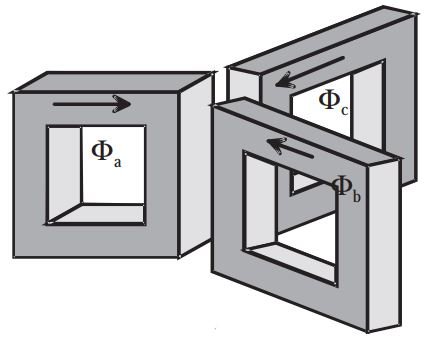
\includegraphics[width = \linewidth]{trafo-secuencia-1}
		\caption{}
		\label{fig:secuencia-1}
	\end{subfigure}
	\begin{subfigure}[b]{.2\linewidth}
		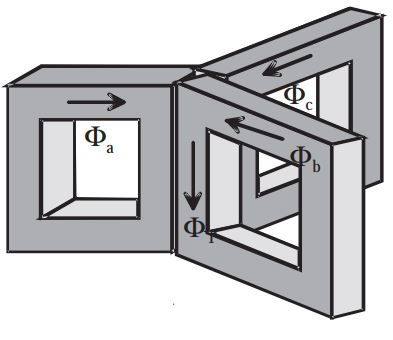
\includegraphics[width = \linewidth]{trafo-secuencia-2}
		\caption{}
		\label{fig:secuencia-2}
	\end{subfigure}
	\begin{subfigure}[b]{.2\linewidth}
		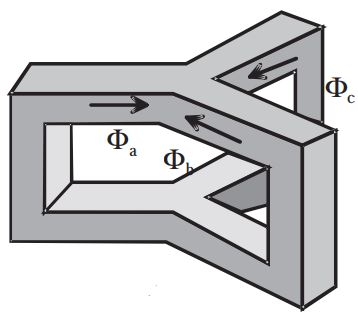
\includegraphics[width = \linewidth]{trafo-secuencia-3}
		\caption{}
		\label{fig:secuencia-3}
	\end{subfigure}
	\caption{Génesis de un trafo trifásico a partir de tres monofásicos.}
	\label{fig:trafo-secuencia}
\end{figure}

\subsubsection{Análisis de funcionamiento}


En este estudio \textbf{hay que considerar cada columna como un transformador monofásico}, pudiéndose aplicar el mismo análisis visto en secciones precedentes.
Además, hay que tener presente que los devanados primario y secundario de una misma columna \textbf{están en fase}. Por ejemplo,
la relación de transformación será el cociente entre el número de espiras \textbf{por fase} del primario y el número de espiras \textbf{por fase} del secundario, que coincidirá con la relación entre las \textbf{f.e.m.s. por fase entre primario y secundario}.\\ %Revisar

Se emplearan las letras $A$, $B$, $C$ para las denominaciones de los devanados primarios o de A.T. y $a$, $b$, $c$, indicarán los terminales de la misma polaridad en el devanado secundario o de B.T., como muestra en la \ref{fig:trafo-trifasico}.\\

Las formas que más frecuentemente se emplean para realizar las conexiones de los arrollamientos son en \textbf{estrella}, en \textbf{triángulo}, y en \textbf{zig-zag}, aunque en esta última no se profundiza en \materia. Dependiendo del tipo de conexión en los devanados, pueden aparecer unas diferencias de fase entre las tensiones compuesta de primario y secundario.

\begin{figure}[H]
	\centering
	\begin{subfigure}[b]{.2\linewidth}
		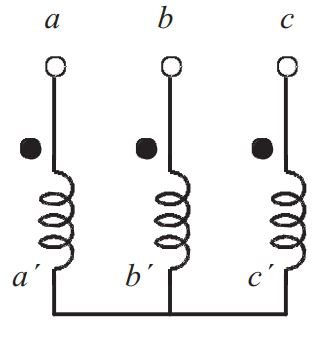
\includegraphics[width = \linewidth]{estrella}
		\caption{Estrella}
	\end{subfigure}
	\begin{subfigure}[b]{.2\linewidth}
		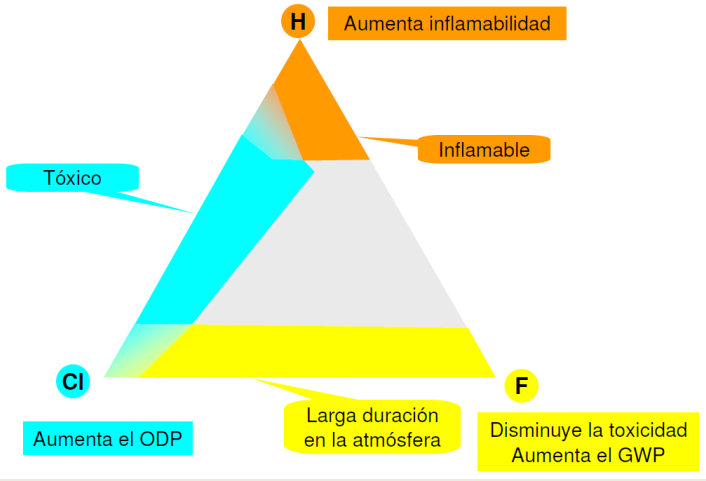
\includegraphics[width = \linewidth]{triangulo}
		\caption{Triángulo o Delta}
	\end{subfigure}
	\begin{subfigure}[b]{.2\linewidth}
		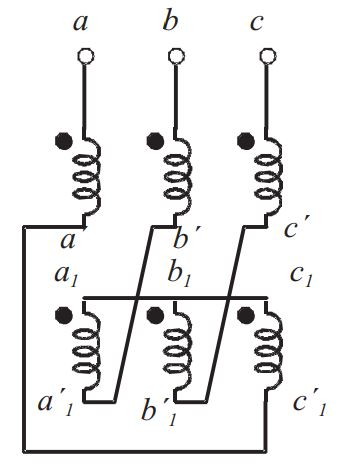
\includegraphics[width = \linewidth]{zigzag}
		\caption{Zig-zag}
	\end{subfigure}
	\caption{Tipos de conexiones de los transformadores trifásicos.}
\end{figure}

\subsubsection{Índice horario del transformador}